
    
\begin{frame}{Pursuit Evasion Game} 

    \begin{figure}
        \centering
        \begin{minipage}{0.49\linewidth}
            \centering
            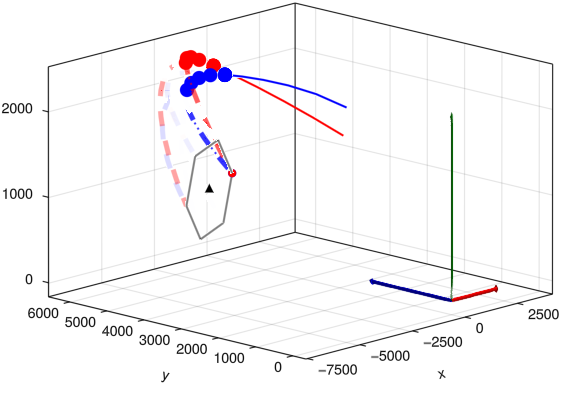
\includegraphics[width=\linewidth]{images/k_replan_1.png}
            \caption{First planning period}
            \label{fig:replan_1}
        \end{minipage}
        \hfill
        \begin{minipage}{0.49\linewidth}
            \centering
            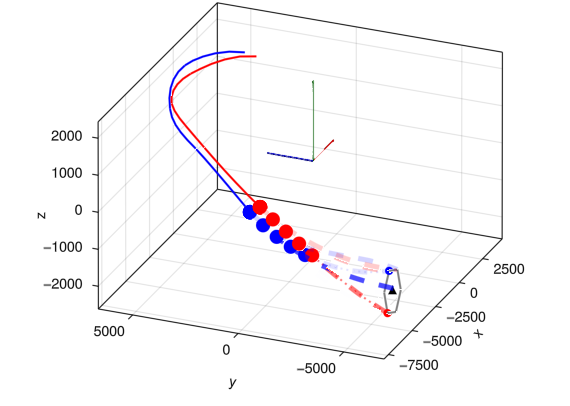
\includegraphics[width=\linewidth]{images/k_replan_5.png}
            \caption{Fifth planning period}
            \label{fig:replan_5}
        \end{minipage}
    \end{figure}
    

    % \begin{figure}
    %     \centering
    %     \includegraphics[width=0.5\linewidth]{pres_images/k_replan_1.png}
    %     \caption{First planning period}
    %     \label{fig:enter-label}
    % \end{figure}

    % \begin{figure}
    %     \centering
    %     \includegraphics[width=0.5\linewidth]{pres_images/k_replan_5.png}
    %     \caption{Fifth planning period}
    %     \label{fig:enter-label}
    % \end{figure}
    
\end{frame} 

\begin{frame}{Pursuit Evasion Game}

    However, when I ran a unit test, encountered something concerning: 
    \begin{itemize}
        \item P1 hard-coded to choose Vertex 1 
        \item P2 greedy SHOULD capture, thus player distance should \rightarrow 0 
    \end{itemize}

    \begin{figure}
        \centering
        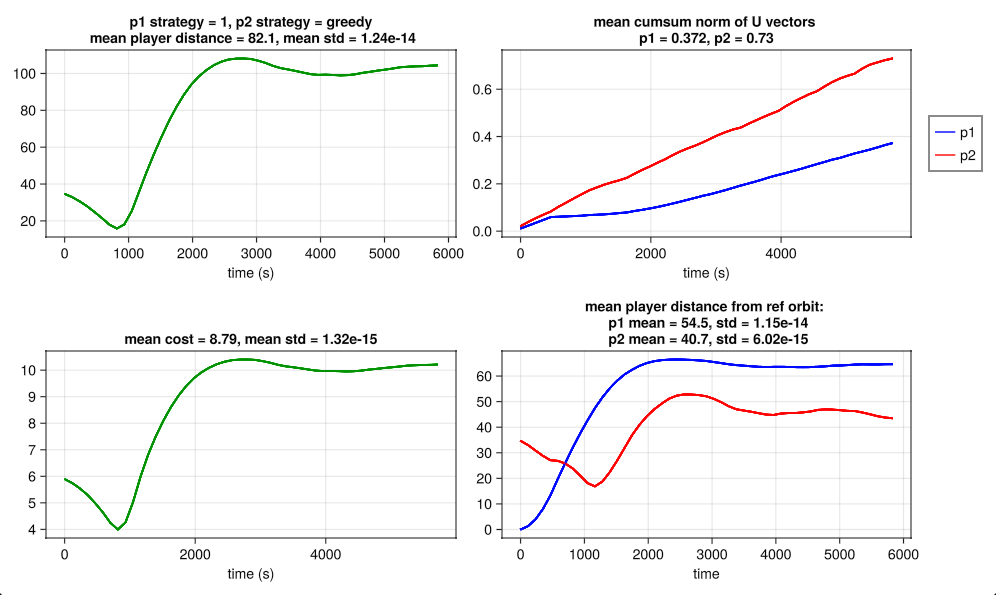
\includegraphics[width=0.7\linewidth]{pres_images/p1-1_p2-greedy.png}
        \caption{P1 = Vertex 1, P2 = Greedy. Mean player distance large }
        \label{fig:placeholder}
    \end{figure} 

\end{frame}

\begin{frame}{Fictitious Play }

    \textbf{Solution:} Instead of assuming perfect play, each player will maintain a belief about the other's behavior based on past observations and play the Best Response to that belief. 

    Instead of assuming perfect play (always choose greedy policy) 
% 
    \begin{align}
        \max_{ \mathbf{z} \in \mathbb{R}^6 }    & \; \; \mathbf{1}^T \mathbf{z} \\ 
        \text{ subject to }                     & \; \; \mathbf{1} \geq A^T \mathbf{z}    
    \end{align} 

    We exploit the actual response based on belief vector $\hat{q}$, the empirical frequency of the other player's past responses 
    % 
    \begin{equation}
        \max_{i} \sum_{j=1}^6 A_{ij} \hat{q}_j
    \end{equation}
    
\end{frame}

\begin{frame}{Fictitious Play }

    With belief vector added to optimization problem: 
    \begin{itemize}
        \item P1 hard-coded to choose Vertex 1 
        \item P2 FP best response results in player distance \rightarrow 0: capture 
    \end{itemize}

    \begin{figure}
        \centering
        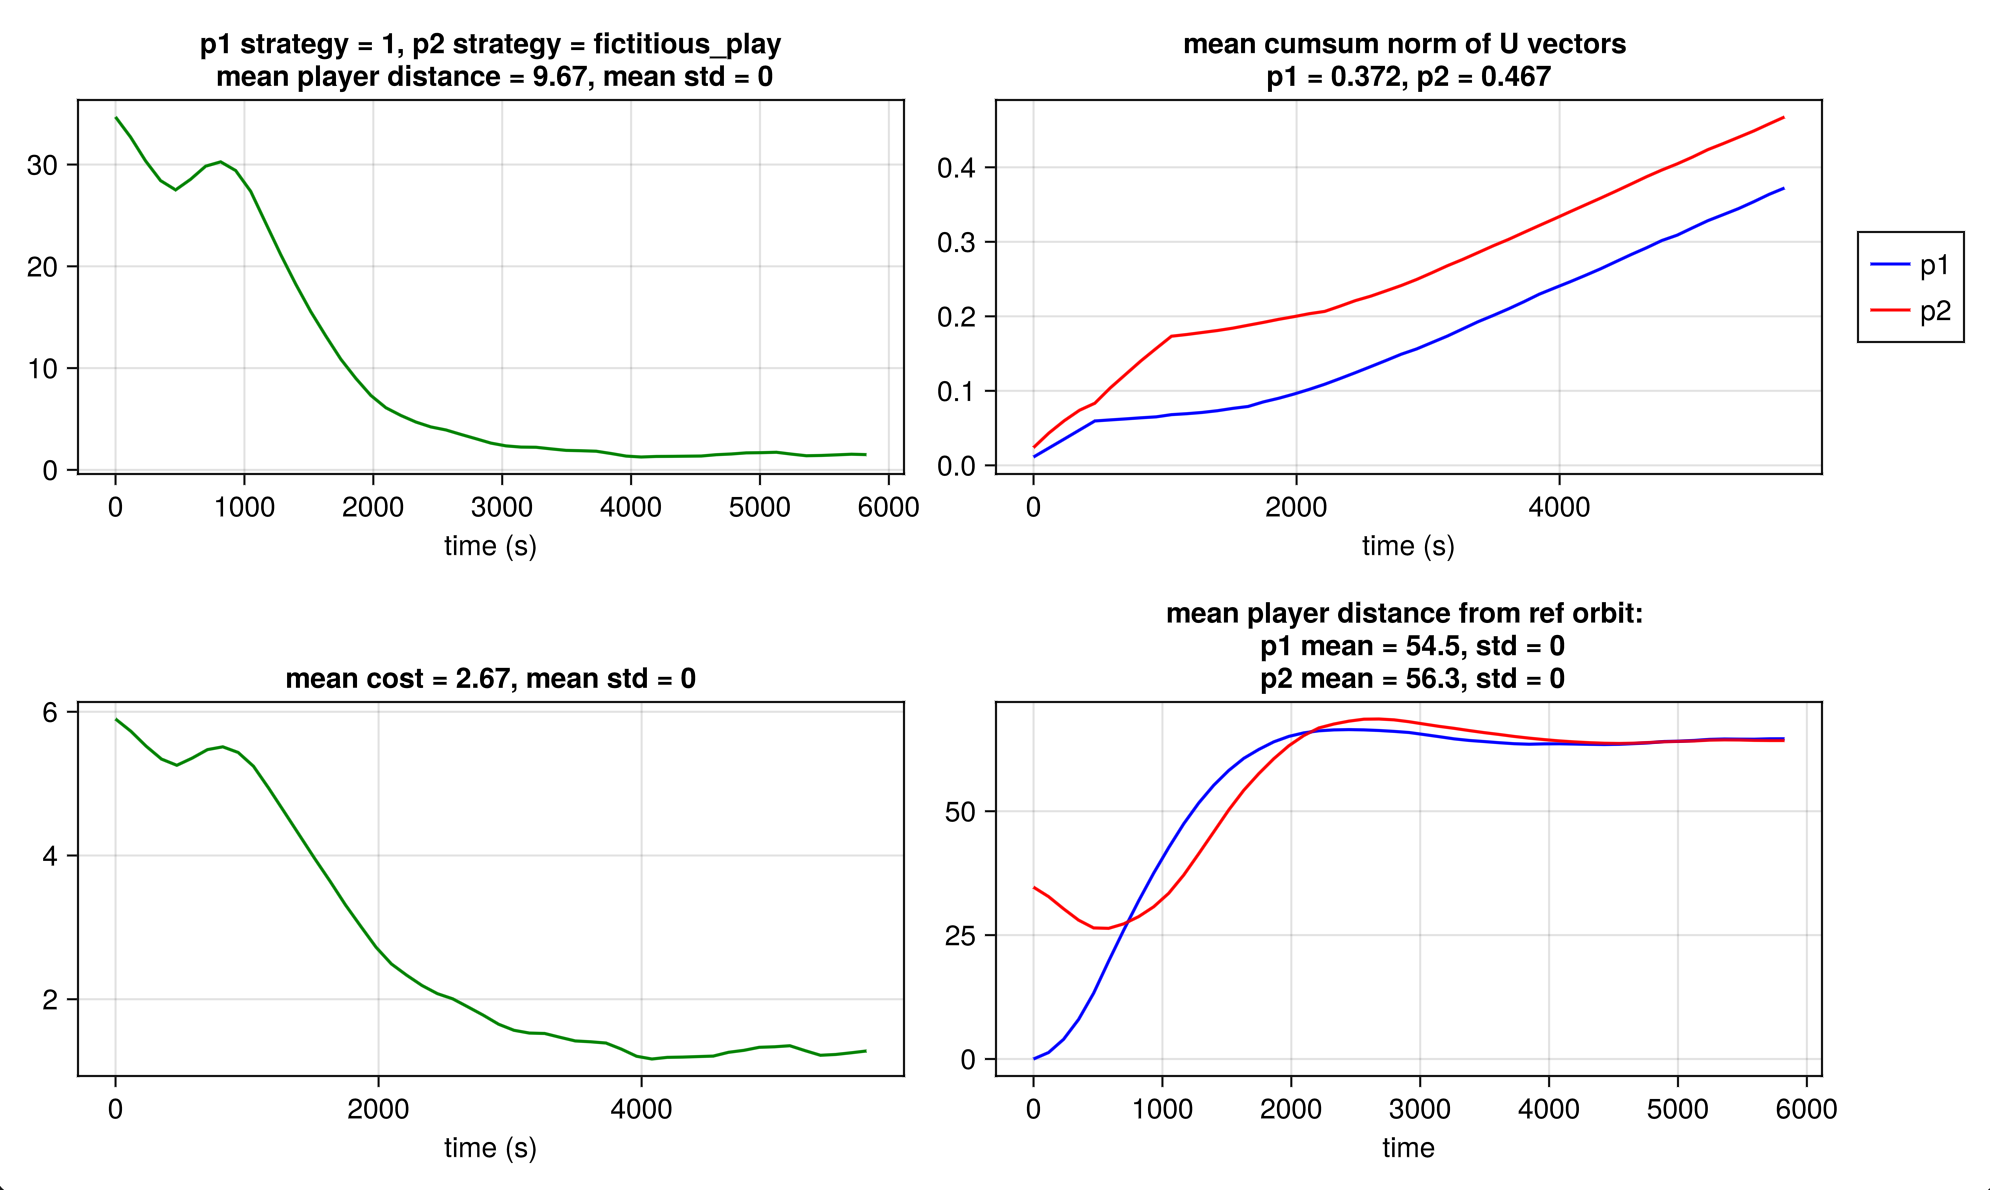
\includegraphics[width=0.7\linewidth]{pres_images/p1-1_p2-fp-greedy.png}
        \caption{P1 = Vertex 1, P2 = Fictious Play. Mean player distance \rightarrow 0 }
        \label{fig:placeholder}
    \end{figure}
    
\end{frame}

% ------

\begin{frame}{Monte Carlos }

    \begin{columns}
        \begin{column}{0.5\textwidth}
            \begin{figure}
                \centering
                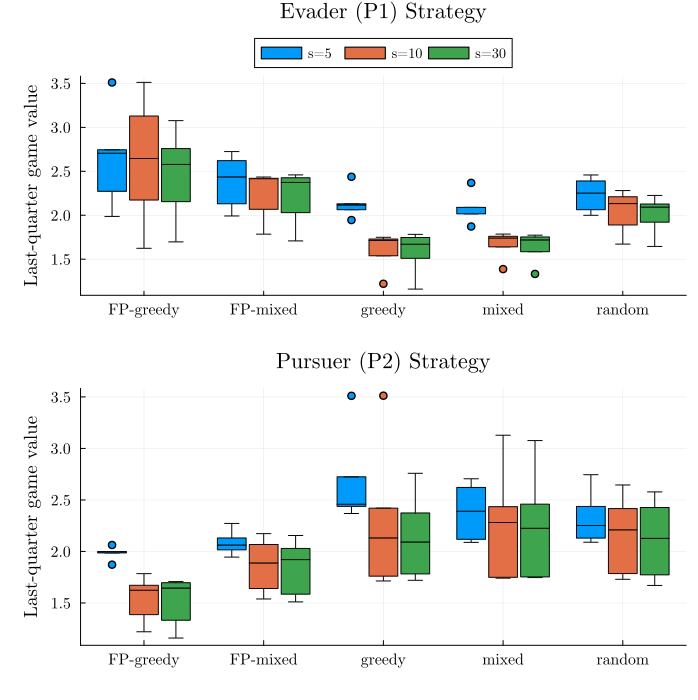
\includegraphics[width=\linewidth]{images/MC_results_late_game_boxplot.png}
                \caption{Averaged game values for each strategy}
                \label{fig:placeholder}
            \end{figure}
        \end{column}
        \begin{column}{0.5\textwidth}
            \begin{figure}
                \centering
                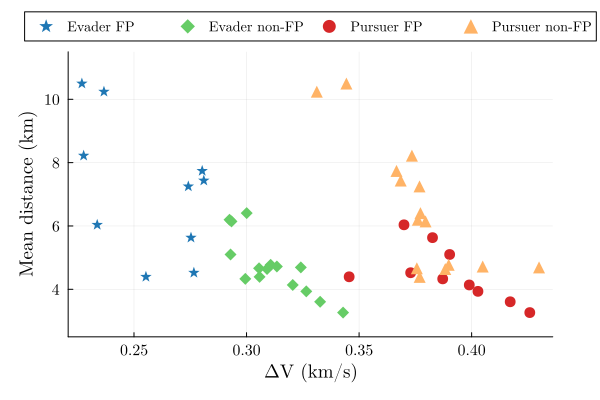
\includegraphics[width=\linewidth]{images/MC_results_late_game_delta_v_vs_distance.png}
                \caption{Mean distance vs. cumulative $\Delta V$ for each strategy}
                \label{fig:placeholder}
            \end{figure}
        \end{column}
    \end{columns}
    
\end{frame}

% ------

\begin{frame}{Monte Carlos }

    \begin{figure}
        \centering
        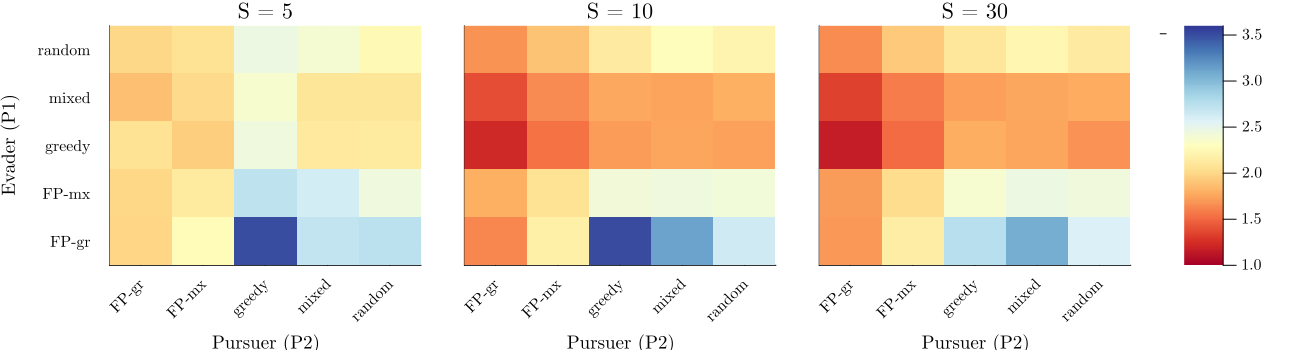
\includegraphics[width=\linewidth]{images/MC_results_late_game_heatmap.png}
        \caption{Meta-game Nash Equilibrium: P1 = FP-greedy, P2 = FP-greedy. Evader: blue is better (higher). Pursuer: red is better (lower). }
        \label{fig:placeholder}
    \end{figure}
    
\end{frame}

% \begin{frame}{Pursuit Evasion Game }

%     Alternately, instead of sampling from the distribution, we can choose to always pick the highest weight trajectory (pure), or we can choose a trajectory completely randomly disregarding weights. Here are monte Carlo results from running 100 simulations of each case. 

%     \begin{figure}
%         \centering
%         \begin{minipage}{0.32\linewidth}
%             \centering
%             \includegraphics[width=\linewidth]{pres_images/pure.png}
%             \caption{Pure Strategy}
%             \label{fig:pure}
%         \end{minipage}
%         \hfill
%         \begin{minipage}{0.32\linewidth}
%             \centering
%             \includegraphics[width=\linewidth]{pres_images/random.png}
%             \caption{Random Strategy}
%             \label{fig:random}
%         \end{minipage}
%         \hfill
%         \begin{minipage}{0.32\linewidth}
%             \centering
%             \includegraphics[width=\linewidth]{pres_images/mixed.png}
%             \caption{Mixed Strategy}
%             \label{fig:mixed}
%         \end{minipage}
%     \end{figure}
    
% \end{frame}

